\begin{figure}[h!]
   \centering
   \begin{subfigure}[b]{0.6\textwidth}
      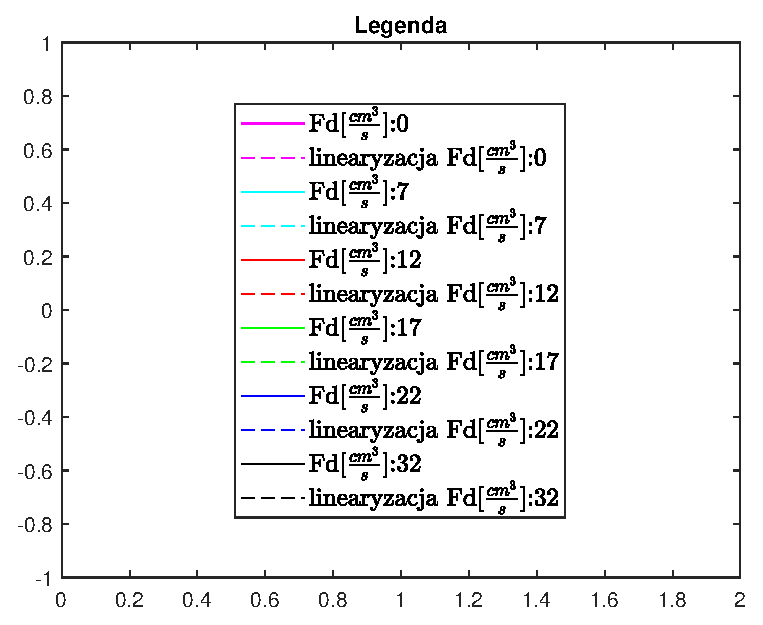
\includegraphics[width=1\linewidth]{img/step-responses-fd/legendFigureFd.eps}
      \caption{}
      \label{fig:fig:stepResponsesFhFd1}
   \end{subfigure}
       
   \begin{subfigure}[b]{0.6\textwidth}
      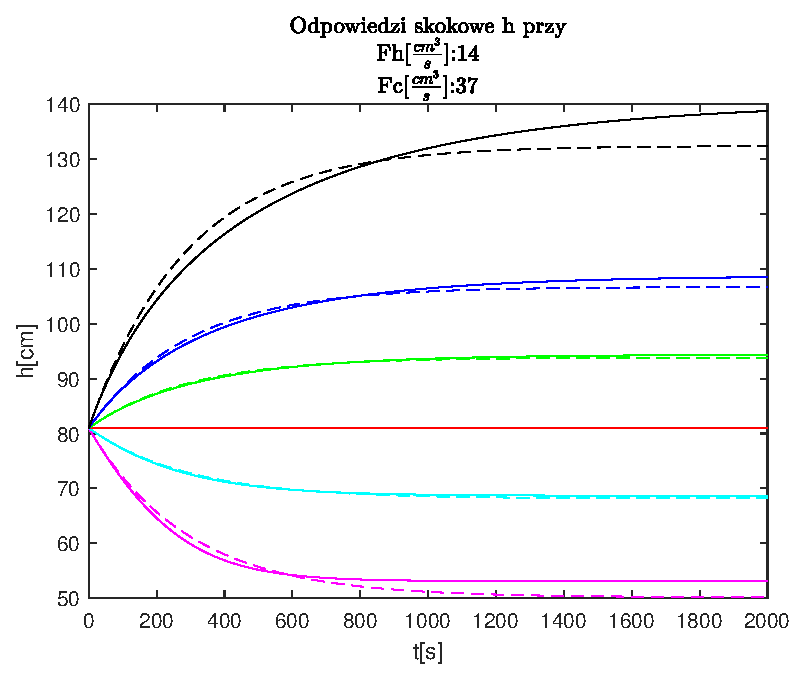
\includegraphics[width=1\linewidth]{img/step-responses-fd/stepResponseHFhFd.eps}
      \caption{}
      \label{fig:fig:stepResponsesFhFd2}
   \end{subfigure}
       
   \begin{subfigure}[b]{0.6\textwidth}
      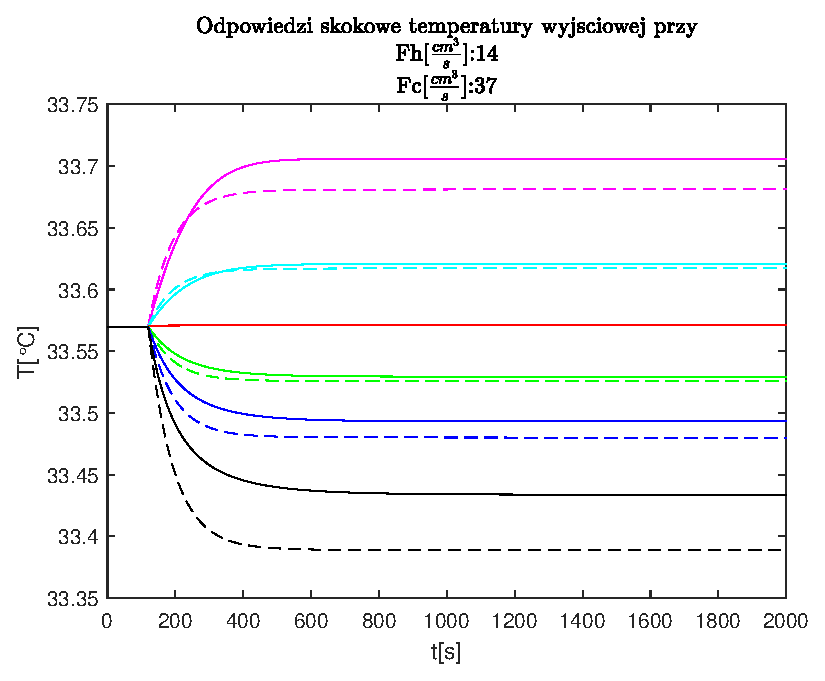
\includegraphics[width=1\linewidth]{img/step-responses-fd/stepResponseToutFhFd.eps}
      \caption{}
      \label{fig:fig:stepResponsesFhFd3}
   \end{subfigure}
       
   \begin{subfigure}[b]{0.6\textwidth}
      \includegraphics[width=1\linewidth]{img/step-responses-fd/stepResponseUFd.eps}
      \caption{}
      \label{fig:fig:stepResponsesFhFd4}
   \end{subfigure}
       
   \caption{Wykresy dla zakłócenia Fd przy Fh[$\frac{cm^3}{s}$]: 14 i  Fc[$\frac{cm^3}{s}$]: 37}
   \label{fig:stepResponsesFhFd}
\end{figure}
           
